\documentclass[pdftex,10pt,a4paper,oneside]{report}

\usepackage{amsmath}
\usepackage{amssymb}
\usepackage{amsfonts}
\usepackage{algorithm}
\usepackage{algorithmic}
\usepackage{fancyhdr}
\usepackage{graphicx}
\usepackage{lipsum}
\usepackage{multirow}
\usepackage{setspace}
\usepackage{verbatim}
\usepackage{standalone}
\usepackage{tabularx}
\usepackage{pgfplots}
\usepackage{etoolbox} % 引入 etoolbox 宏包
\usepgfplotslibrary{groupplots}
\pgfplotsset{compat=1.18}

\fancyhf{}
\pagestyle{fancy}
\renewcommand{\headrulewidth}{0.2pt}

% Styles can be Sonny, Lenny, Glenn, Conny, Rejne, Bjarne and Bjornstrup
\raggedbottom
\setcounter{topnumber}{5}
\setcounter{bottomnumber}{5}
\setcounter{totalnumber}{10}
\renewcommand{\topfraction}{0.95}
\renewcommand{\bottomfraction}{0.95}
\renewcommand{\textfraction}{0.05}
\renewcommand{\floatpagefraction}{0.95}
\usepackage[Sonny]{fncychap}
\usepackage[font=small,labelfont=bf]{caption}
\captionsetup{skip=2pt} % caption与内容间距
\setlength{\textfloatsep}{3pt plus 2pt minus 1pt} % 图/表与正文间
\setlength{\floatsep}{3pt plus 1pt minus 1pt}     % 两个浮动体之间
\setlength{\intextsep}{3pt plus 1pt minus 1pt}    % 文中浮动体与正文
% 定义一个命令来应用所有参考文献格式
\newcommand{\setupbib}{%
	\small % 1. 设置字体大小为 \small
	% 你也可以用 \footnotesize, \scriptsize 等
	
	\setlength{\itemsep}{0pt} % 2. 设置条目之间的垂直间距
	% 设置为 0pt 表示移除额外的间距，只保留基线间距。你也可以设为 2pt, 5pt 等来增加间距。
	
	\setlength{\parskip}{0pt} % 3. 设置条目内部段落的间距（对于有多个段落的条目）
}

% 在 thebibliography 环境开始时，自动执行 \setupbib 命令
\AtBeginEnvironment{thebibliography}{\setupbib}
\begin{document}

% !TEX root =  ../Dissertation.tex

\thispagestyle{empty}

\begin{spacing}{2}
	\begin{center}
		
\includegraphics[scale = 1.5]{Preamble/BirmCrest.png}
	\end{center}
	\vspace{10mm}

	\begin{center}
		\textbf{\large A Study on Speech Emotion Recognition Based on Multi-Feature and Deep Models}
		\vspace{20mm}
		\\\textbf{\Large By}
		\\\textbf{\Large Mian Li}
	    \\\text{\Large Student ID: 2773117}
	    \\\text{\Large Supervisor: Dr. Rishiraj Bhattacharyya}
		\vspace{30mm}
		
	\end{center}
	\begin{center}
		{\large School of Computer Science}
		\\ {\large College of Engineering and Physical Sciences}
		\\ {\large University of Birmingham}
		\\ {\large 2024-25}
	\end{center}
\end{spacing}

\pagenumbering{roman}



\chapter*{Abstract}
\addcontentsline{toc}{chapter}{Abstract}

This dissertation addresses the critical challenge of robust Speech Emotion Recognition (SER) in the presence of environmental noise. While deep learning has significantly advanced SER, model performance often degrades when moving from clean, laboratory-recorded data to more realistic, noisy conditions. This study conducts a systematic evaluation of deep learning models and audio features to improve noise robustness and generalization. We investigate four distinct architectures: a Multilayer Perceptron (MLP), a shallow Convolutional Neural Network (CNN), a deeper ResNet-18, and the attention-based Audio Spectrogram Transformer (AST). These models are trained on both traditional Mel-frequency cepstral coefficient (MFCC) features and 2D Mel-spectrograms.

The core of our methodology revolves around a comprehensive on-the-fly data augmentation strategy, where training data is mixed with white noise and natural soundscapes from the ESC-50 dataset at various signal-to-noise ratios (SNRs). We evaluate model performance on two standard benchmarks, RAVDESS and IEMOCAP, under both clean and noisy test conditions. The findings consistently demonstrate that the AST architecture surpasses the convolutional and MLP-based models, particularly when trained with data augmentation. Augmentation not only preserves but often improves AST's performance on clean test sets while significantly enhancing its robustness against a wide range of noises and SNRs.

Furthermore, our analysis reveals a crucial interaction between model architecture and augmentation strategy. While AST effectively leverages diverse acoustic perturbations to learn noise-invariant features, the ResNet-18 model proves more fragile, exhibiting performance degradation under the same conditions. The study also highlights dataset-specific effects, where augmentation leads to a more balanced precision-recall trade-off on the heterogeneous IEMOCAP dataset, particularly for the AST model. Ultimately, this research underscores the synergy between transformer architectures and robust data augmentation, presenting a promising framework for developing more practical and generalizable SER systems.
%\include{Preamble/Dedication} % Comment out for UG dissertations

\chapter*{Acknowledgements}
\addcontentsline{toc}{chapter}{Acknowledgements}

Time has flown by, and my master’s journey has now reached its conclusion. Along this path, I have been fortunate to meet many people and experiences that I will always cherish.

First and foremost, I would like to express my deepest gratitude to my supervisor, Dr. Rishiraj Bhattacharyya, for his patient guidance and invaluable support throughout my research and writing. His calm attitude and rigorous academic spirit have not only provided me with direction but also given me the confidence to overcome challenges along the way.

I am equally grateful to all the sincere and wonderful friends I met during my year in the UK. You made life in a foreign country warm and memorable, turning ordinary days into something bright with kindness and laughter.

I would also like to thank myself—for making the choice to pursue this path and for holding on with persistence. And to my parents, whose understanding and unconditional support have always been my strongest foundation, I owe more than words can express.

Life is a continuous journey forward, and the future shines with light. May we all carry hope in our hearts, live fully in the present, and embrace the bright days ahead.
% !TEX root =  ../Dissertation.tex

\chapter*{Declarations}
\addcontentsline{toc}{chapter}{Declarations}
I certify that this project is my own work. Code development was assisted by Claude Sonnet 3.7 and debugging by ChatGPT 4.0. The report structure and initial drafts are mine; final editing was assisted by ChatGPT for clarity and consistency. All outputs have been reviewed and edited to accurately reflect my work. % Comment out for UG dissertations
%\include{Preamble/Sponsors} % Comment out for UG dissertations

\chapter*{Abbreviations}
\addcontentsline{toc}{chapter}{Abbreviations}

\begin{flushleft}

AST \hfill Audio Spectrogram Transformer

CCC \hfill concordance correlation coefficient

CNN \hfill convolutional neural network

DCT \hfill discrete cosine transform

DFT \hfill discrete Fourier transform

DTs \hfill Decision Trees

FFN \hfill Feed-forward network

GMMs \hfill Gaussian Mixture Models

HMMs \hfill Hidden Markov Models

HSFs \hfill high-level functional statistics

KNN \hfill K-nearest neighbors

LLDs \hfill low-level descriptors

MFCCs \hfill Mel-frequency cepstral coefficients

MHSA \hfill multi-head self-attention

MLP \hfill multilayer perceptron

RMS \hfill root-mean-square

SER \hfill Speech Emotion Recognition

SNR \hfill signal-to-noise ratio

SVMs \hfill Support Vector Machines

TEO \hfill Teager Energy Operator

UAR \hfill unweighted average recall

ViT \hfill Vision Transformer

\end{flushleft}
%\include{Preamble/Notations} % Comment out for most dissertations
\include{Preamble/Contents}
\include{Preamble/Lists}
\include{Preamble/ChapterMods}

\include{Chapter1/Chapter1}
% !TEX root =  ../Dissertation.tex

\chapter{Literature Review}








\section{Datasets for Speech Emotion Recognition}

Datasets are foundational to empirical research in Speech Emotion Recognition (SER). They can be broadly categorized into acted corpora and spontaneous or in-the-wild corpora. Acted datasets are typically recorded in controlled laboratory environments with professional actors performing target emotions. While these corpora offer clean signals and clearer affective cues that facilitate modeling, they may over-represent exaggerated expressions and fail to capture the subtleties of everyday speech. By contrast, spontaneous corpora contain naturalistic affect produced in real interactions or semi-scripted dialogues. They better reflect practical deployment scenarios but introduce additional challenges such as background noise, speaker overlap, label ambiguity, and class imbalance. Below we summarize several widely used SER datasets.

\textbf{RAVDESS.} The Ryerson Audio-Visual Database of Emotional Speech and Song contains recordings from 24 professional actors (12 female, 12 male) producing two lexically matched statements across eight emotions (neutral, calm, happy, sad, angry, fearful, disgust, surprise) with normal and strong intensities (neutral has no intensity). The speech subset totals 1,440 audio files, recorded with consistent studio conditions, and is commonly used for speaker-independent evaluation. RAVDESS provides balanced classes and clear prosodic cues, making it suitable for benchmarking and ablation studies; however, its acted nature can limit ecological validity when models are deployed on spontaneous speech.

\textbf{IEMOCAP.} Collected at the University of Southern California, IEMOCAP is a multimodal corpus containing speech, video, facial motion capture, and transcripts over approximately 12 hours of dyadic interactions with 10 actors (five female, five male) arranged into five sessions (each session features one female–male pair). The corpus includes both scripted and improvised dialogues. Utterances are annotated by multiple raters for nine discrete emotions (anger, happiness, excitement, sadness, frustration, fear, surprise, neutral, and other) as well as three continuous dimensions (valence, arousal, dominance). In practice, many studies merge excitement into happiness, yielding a four-class set (neutral, angry, happy, sad) or a six-class set (neutral, angry, happy, sad, frustration, surprise). For comparability, this thesis adopts both the four-class and six-class protocols in line with prior work.

\textbf{EmoDB.} The Berlin Database of Emotional Speech comprises recordings from 10 German actors (five female, five male) who produced 10 phonetically balanced sentences with seven target emotions: anger, sadness, happiness, fear, neutral, disgust, and boredom. After rigorous quality screening, around 500 utterances were retained. Audio was recorded in a studio at 48 kHz, 16-bit, and is often downsampled to 16 kHz for processing. Although acted, the dataset emphasizes natural-sounding realizations through actor induction techniques, providing strong, well-separated emotional prototypes.

\textbf{MELD.} The Multimodal EmotionLines Dataset extends EmotionLines by adding audio and video modalities to textual dialogues. Derived from the TV show “Friends,” MELD contains over 1,400 multi-speaker conversations and more than 13,000 utterances, annotated with seven emotions: anger, disgust, sadness, joy, neutral, surprise, and fear. Its multimodal, conversational structure enables the study of contextual emotion dynamics and speaker interactions beyond isolated utterances.

\section{SER with Acoustic Features}
Acoustic feature engineering plays a central role in early SER pipelines. It compresses raw waveforms into compact descriptors derived from time-domain and frequency-domain analyses, guided by speech science. Canonical categories include prosodic features (pitch, energy, duration), voice-quality features (jitter, shimmer, harmonicity), spectral features (formants, cepstral coefficients), and Teager Energy Operator (TEO) based features. These low-level descriptors (LLDs) capture frame-wise micro-variations in speech and can be summarized into high-level functional statistics (HSFs) such as means, first- and second-order derivatives, and other moments to encode utterance-level context.

Empirical studies have shown that acoustic features carry substantial affective information, reflecting changes in emotion, speaker identity, speaking style, and tempo [41]. As illustrated in Figure 1.2, LLDs and HSFs form the basis of many classical SER systems. Lee et al.  and Schuller et al.  reported strong results using feature sets combining energy-, pitch-, and spectral-related cues, with pitch-related features often proving more discriminative than energy features. Rao et al. [54] compared LLDs against HSFs (and their combination) and found that combining frame-level prosody (e.g., F0 trajectories, energy) with statistical summaries improves recognition performance. Lugger et al.  integrated prosodic and voice-quality features (e.g., glottal gradient, skewness gradient, closure rate gradient) within a two-stage classifier to reach 74.5\% accuracy. Li et al.  further augmented HSFs with jitter and shimmer to boost performance. Zhang et al. combined prosodic with voice-quality features (including the first three formants), improving accuracy by about 10\% over prosody-only baselines. Sato et al.  used clustering to label frames and constructed a segmented MFCC feature set, outperforming KNN on prosody and HMMs on conventional MFCCs. Bitouk et al.  introduced new spectral features by computing MFCCs separately for stressed vowels, unstressed vowels, and consonants, concluding that consonants may carry richer affective cues than vowels. Zhou et al.  proposed three TEO variants—especially a standard-band TEO autocorrelation envelope—to study airflow energy changes under stress, achieving better results than pitch+MFCC combinations.

After feature extraction, classifiers are typically used for final affect prediction. Traditional approaches include Gaussian Mixture Models (GMMs), Support Vector Machines (SVMs), and Decision Trees (DTs) . More recent methods employ deep learning to learn discriminative affect representations from acoustic features, such as 1D CNNs and RNNs, trained with task-appropriate loss functions. Representative studies are summarized in Table 1.1.

Overall, acoustic-feature-based SER offers two key advantages. First, it provides a degree of interpretability: models can assign higher weights to features with stronger affective discriminability, which often aids accuracy compared to purely black-box baselines. Second, system complexity can be relatively low: feature extraction is algorithmic with few learnable parameters, while deep architectures built on these features improve adaptability and reduce overfitting, enabling transfer across related affective tasks. Despite progress, several issues remain: (1) many features rely on the short-time Fourier transform (STFT), a global transform that may inadequately represent the inherently non-stationary, localized time–frequency patterns of affect; (2) attention mechanisms operating on handcrafted features may struggle to highlight truly salient regions, potentially discarding relevant emotional cues.

\section{SER with Spectrogram-based Features}

A central question in spectrogram-based SER is how to extract affectively discriminative representations from time–frequency images. Mel-spectrograms differ from classical handcrafted features (e.g., formants, jitter, MFCCs) in that they preserve localized time–frequency structure and delegate hierarchical feature learning to deep networks. Representing energy over time and frequency in a 2D grid enables learning of complex spectro-temporal patterns that are difficult to encode with fixed handcrafted descriptors [63]. During training, networks can discover filter-like patterns akin to Mel filterbanks while also capturing long-range dependencies and contextual cues typically missed by shallow features.

Since the 2012 deep learning breakthroughs on ImageNet, advances in model capacity and data processing have translated to SER. Compared with conventional machine learning, deep models  can learn affect representations without manual feature selection. Feed-forward deep neural networks (DNNs) comprise multiple hidden layers whose weights are optimized via gradient descent and backpropagation to minimize a task loss. Convolutional neural networks (CNNs) are particularly impactful in SER , as spectrograms exhibit strong local correlations along time and frequency; local receptive fields allow CNNs to extract progressively higher-level features from 2D inputs . Recurrent neural networks (RNNs)  and Long Short-Term Memory (LSTM) networks  are commonly stacked on top of CNN features to model temporal dependencies and can also operate directly on frame-level acoustic features to yield high-level affect representations . Attention mechanisms  further refine these representations by emphasizing salient regions conducive to emotion discrimination.

Rapid progress has been reported in recent years . Trigeorgis et al.  and Lim et al.  proposed CNN–LSTM hybrids in which CNNs extract high-level spectrogram features and LSTMs capture sequence dynamics, outperforming traditional machine learning; similar architectures have been widely adopted. To model spatial relationships in spectra, capsule networks based on CNNs have also been explored , achieving promising sentence-level affect modeling. Representative spectrogram-based deep architectures for SER are summarized in Table 1.2.

On top of high-capacity encoders, attention mechanisms have been extensively used to further improve accuracy , including self-attention, local attention, hop-wise attention, and many other variants . These modules enhance weights of informative time–frequency regions while suppressing irrelevant ones, thereby focusing the network on discriminative patterns; see Table 1.3 for recent studies leveraging attention to boost SER.

Finally, learned affect representations are mapped to task outputs via suitable loss functions and evaluation metrics. For categorical SER, cross-entropy remains the dominant training objective, while mean squared error is often used for dimensional emotion regression. Historically, accuracy was the default metric; however, as datasets grew and class imbalance became prevalent, the Interspeech 2009 Emotion Challenge  popularized unweighted average recall (UAR), computed as the mean of per-class recalls, which is now widely adopted for imbalanced settings. For dimensional SER, the concordance correlation coefficient (CCC)  is commonly used. From Tables 1.3 and 1.4 we observe steady gains from stronger encoders and attention, yet several challenges remain: (1) fixed-size convolutional kernels can restrict the effective receptive field over salient emotional regions, limiting global context capture; (2) attention layers may over-rely on fully connected heads and softmax, under-exploiting local, global, and positional cues; (3) cross-entropy is sensitive to label distributions and can struggle when class manifolds are close; (4) variable-length utterances complicate segment-level training and can misalign segment labels with utterance-level annotations.

\include{Chapter3/Chapter3}
% !TEX root =  ../Dissertation.tex

\chapter{Experiments}

This chapter presents a comprehensive experimental study on SER under clean and noisy conditions. We evaluate multiple architectures and noise augmentation strategies on two datasets, adhering to the unified notation and preprocessing defined in Chapter 3. Unless otherwise specified, audio is sampled at \(f_s\), the time-domain signal is \(x[n]\), noise is \(v[n]\), and on-the-fly mixtures during training follow
\(x_{\mathrm{mix}}[n] = x_s[n] + g\, x_n[n]\) with gain \(g\) computed from target SNR as in Chapter 3.

\section{Common Settings}

\subsection{Datasets and splits}
We use RAVDESS (speech actors 01–24) and IEMOCAP. Data splits follow the established protocol for each dataset. Validation and clean test sets are never augmented; only the training split is subjected to on-the-fly noise mixing when enabled. The batch size of MLP, shallow CNN, and Resnet18 is 128, and 64 for AST. All models are trained using Adam \cite{Kingma2014Adam} optimizer with a initial learning rate of 0.001. The training is terminated when the validation loss does not improve for 10 epochs.

\paragraph{Class schemes and dataset sizes.}
For categorical SER we adopt fixed emotion inventories per corpus.
\begin{itemize}
  \item \textbf{RAVDESS (8 classes).} Neutral, Calm, Happy, Sad, Angry, Fearful, Disgust, Surprised. We use the speech subset from actors 01–24 and retain all eight categories. Splits are speaker-disjoint following the common protocol. Dataset sizes used in this work (utterances): \textit{Train = 1152,  Test = 288}.
  \item \textbf{IEMOCAP (4 classes).} We adopt the standard 4-class mapping with Happy and Excited merged into Happy: Angry, Happy, Sad, Neutral. Sessions are used for speaker-disjoint splits. Dataset sizes (utterances): \textit{Train = 10560, Test = 2896}.
\end{itemize}
These label spaces remain fixed across Experiments A–D. All reported metrics are computed on the same class definitions; no relabeling is performed between experiments.

\subsection{Models}
We compare a convolutional baseline (ResNet-18 on Log-Mel spectrograms) and a transformer-based model (AST Base on filterbank features), alongside lighter baselines where applicable (MLP and shallow CNN) to contextualize complexity–performance trade-offs.

\paragraph{Implementation summary.}
Models are instantiated via a configuration-driven factory in \texttt{models.py}: \texttt{create\_model(config)} reads \texttt{config['training']}

\texttt{['model\_name']} and \texttt{config['models'][...]['type']} to build the requested architecture (MLP, ShallowCNN, ResNet18, AST). Core hyperparameters—including \textit{num\_classes}, dropout rates, hidden sizes, and feature types—are taken from the configuration for reproducibility and easy switching between architectures.

\begin{itemize}
  \item \textbf{MLP (MFCC-based).} Input features are MFCC statistics (per-utterance mean and standard deviation concatenated; dimension \(2\times\textit{input\_size}\)). The backbone is a sequence of \texttt{Linear→ReLU→Dropout} blocks; a final linear classifier produces emotion logits. This baseline targets low-dimensional hand-crafted features with small parameter count and stable training.
  \item \textbf{Shallow CNN (Log-Mel-based).} The convolutional trunk has three blocks with channels \(32\to64\to128\). Each block applies \texttt{Conv2d + BatchNorm + ReLU + MaxPool}; an adaptive global average pooling aggregates time–frequency features. A dropout layer and a single \texttt{Linear} head complete classification. The design is lightweight yet effective for 2D time–frequency modeling.
  \item \textbf{ResNet-18 (Log-Mel-based).} The network begins with a \(7\times7\) convolution and max-pooling, followed by four residual stages (channels \(64/128/256/512\), increasing strides). Each \textit{BasicBlock} uses two \(3\times3\) convolutions with identity/projection shortcuts. After adaptive average pooling, a fully connected layer outputs logits. Kaiming initialization and BatchNorm parameter initialization are used; \texttt{num\_classes} is validated at construction.
  \item \textbf{AST (Audio Spectrogram Transformer).} Implemented in \texttt{ast\_model.py} using a DeiT/ViT variant (via \texttt{timm}). \textit{PatchEmbed} is adapted for single-channel Log-Mel; 3-channel weights are merged to 1-channel, and patch grid plus positional embeddings are recomputed (bilinear interpolation or cropping) to match audio shapes. ImageNet pretraining is supported (optionally AudioSet). The head is \texttt{LayerNorm + Linear}. A wrapper (e.g., \texttt{RAVDESSASTModel}) derives input time steps from sampling rate, duration, and \(n\_\mathrm{mels}\), instantiating AST accordingly. Forward path: reshape \((B,T,F)\to(B,1,F,T)\), apply patch embedding, add \texttt{[cls]/[dist]} tokens and positional encodings, pass transformer blocks and normalization, then pool \texttt{cls}/\texttt{dist} representations and use an MLP head to obtain logits.
\end{itemize}



\subsection{Training and evaluation}
Training uses mini-batch stochastic optimization with standard regularization. Metrics on the validation set include accuracy, precision, recall, and macro-F1. Confusion matrices are reported to analyze class-wise separability. Robustness is further assessed on noisy test sets created by offline mixing of \(x[n]\) with held-out noise at specified SNRs \(\in \{0,5,10,20\}\,\mathrm{dB}\). All experiments fix a base random seed 42 unless otherwise stated.

\subsection{Noise augmentation policy}
When enabled, augmentation follows Chapter 3: with probability \(p_{\mathrm{aug}}\), we sample a noise type (white or ESC-50 subsets), sample SNR from \(\{0,5,10,20\}\,\mathrm{dB}\), time-align noise to the utterance, compute gain \(g\) via RMS matching to satisfy the target SNR, form \(x_{\mathrm{mix}}[n]\), apply peak limiting at \(-1\,\mathrm{dBFS}\), and optionally mean–variance normalize prior to feature extraction.

\section{Experiment A: Clean Baselines}
\textbf{Objective.} Establish upper bounds under matched clean conditions to isolate modeling capacity from noise robustness. These baselines indicate how well each architecture fits clean speech and provide a reference point for subsequent robustness interventions.

\textbf{Setup.} All training, validation, and test audio remain unaltered. Feature pipelines follow Chapter 3 (MFCC and log-mel) as required by each model. Optimization hyperparameters are fixed across runs for comparability. No augmentation, denoising, or calibration is applied. Training–validation trajectories are examined to gauge overfitting and learning dynamics.

\textbf{Evaluation.} We report accuracy, precision, recall, and macro-F1, with confusion matrices to visualize class confusability. Macro-F1 is emphasized due to class imbalance, ensuring that performance is not dominated by frequent emotions. Where informative, we comment on calibration and thresholding effects.

\textbf{Results and analysis.} Results of Experiment A on RAVDESS and IEMOCAP are shown in Table \ref{tab:ravdess_results} and Table \ref{tab:iemocap_results} respectively. Figure \ref{fig:expA_barplots} provides a more intuitive view of the results. On RAVDESS, AST Base achieves the best performance (Acc 0.718, Macro-F1 0.714), closely followed by ResNet-18 (Acc 0.687). MLP offers a moderate reference (Acc 0.451), while the shallow CNN underfits substantially (Acc 0.208), suggesting inadequate receptive-field depth for clean spectral patterns. On IEMOCAP, AST again leads in accuracy (0.615) but exhibits a precision–recall asymmetry (Precision 0.682 vs. Recall 0.413), indicative of conservative predictions that miss minority or ambiguous classes. ResNet-18 is competitive yet shows greater variability across sessions, and MLP/CNN display sensitivity to the dataset’s heterogeneity and longer utterances. Confusions concentrate among emotions with overlapping prosody (e.g., neutral–sad, angry–excited), consistent with prior findings. Training–validation comparisons suggest mild overfitting for deeper models on RAVDESS and larger variance on IEMOCAP, pointing to limited per-class data. These ceilings highlight headroom primarily in recall on IEMOCAP and in narrowing the AST–ResNet gap on RAVDESS.





\begin{table}[htbp]
    \centering
    \caption{ Results of Experiment A on RAVDESS}
    \label{tab:ravdess_results}
    \begin{tabular}{lcccc}
        \hline
        Model & Accuracy & Precision & Recall & Macro-F1 \\
        \hline
        MLP & 0.451 & 0.412 & 0.431 & 0.402 \\
        Shallow CNN & 0.208 & 0.141 & 0.192 & 0.127 \\
        ResNet-18 & 0.687 & 0.694 & 0.697 & 0.682 \\
        AST Base &  0.718 &  0.735 & 0.719 & 0.714 \\
        \hline
    \end{tabular}
\end{table}

\begin{table}[htbp]
    \centering
    \caption{ Results of Experiment A on IEMOCAP}
    \label{tab:iemocap_results}
    \begin{tabular}{lcccc}
        \hline
        Model & Accuracy & Precision & Recall & Macro-F1 \\
        \hline
        MLP & 0.583 & 0.498 & 0.342 & 0.340 \\
        Shallow CNN & 0.583 & 0.546 & 0.449 & 0.415 \\
        ResNet-18 & 0.570 & 0.388 & 0.475 & 0.406 \\
        AST Base & 0.615 & 0.682 & 0.413 &  0.448\\

        \hline
    \end{tabular}
\end{table}


\begin{figure}[htbp]
    \centering
    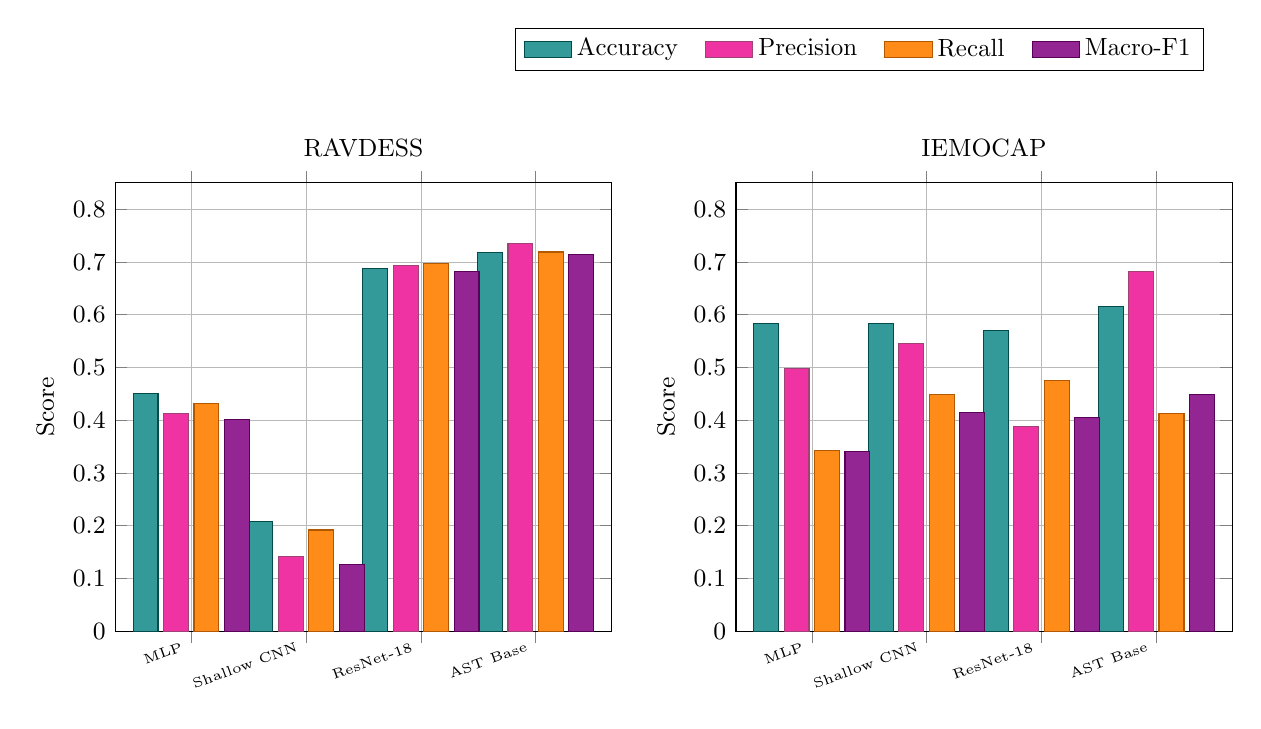
\begin{tikzpicture}
    \pgfplotsset{compat=1.18}

    \begin{groupplot}[
      group style={group size=2 by 1, horizontal sep=4.5em},
      width=0.65\textwidth, height=0.60\textwidth,
      ymin=0, ymax=0.85,
      ymajorgrids, grid=both,
      grid style={line width=.1pt, draw=gray!30},
      major grid style={line width=.2pt, draw=gray!55},
      xtick=data,
      symbolic x coords={MLP, Shallow CNN, ResNet-18, AST Base},
      xticklabel style={font=\tiny, rotate=20, anchor=east},
      ylabel={Score},
      enlarge x limits=0.22,
      ytick distance=0.1,
      ticklabel style={font=\small},
      label style={font=\small}
    ]

    % ---------------- RAVDESS ----------------
    \nextgroupplot[
      title={RAVDESS}, title style={font=\small},
      ybar,
      bar width=9pt,
      legend style={
        at={(1.5,1.25)}, anchor=south,
        nodes={scale=0.9, transform shape},
        legend columns=4, /tikz/every even column/.style={column sep=0.8em},
        row sep=2pt
      }
    ]
    % Accuracy
    \addplot+[draw=teal!60!black, fill=teal!80!white,area legend,
    %   every node near coord/.append style={font=\scriptsize, /pgf/number format/fixed, /pgf/number format/precision=2, yshift=1.5pt}
    ] coordinates
    {(MLP,0.451) (Shallow CNN,0.208) (ResNet-18,0.687) (AST Base,0.718)};
    \addlegendentry{Accuracy}
    % Precision
    \addplot+[draw=magenta!60!black, fill=magenta!80!white,area legend,
      every node near coord/.append style={font=\scriptsize, /pgf/number format/fixed, /pgf/number format/precision=2, yshift=1.5pt}
    ] coordinates
    {(MLP,0.412) (Shallow CNN,0.141) (ResNet-18,0.694) (AST Base,0.735)};
    \addlegendentry{Precision}
    % Recall
    \addplot+[draw=orange!70!black, fill=orange!90!white,area legend,
      every node near coord/.append style={font=\scriptsize, /pgf/number format/fixed, /pgf/number format/precision=2, yshift=1.5pt}
    ] coordinates
    {(MLP,0.431) (Shallow CNN,0.192) (ResNet-18,0.697) (AST Base,0.719)};
    \addlegendentry{Recall}
    % Macro-F1
    \addplot+[ draw=violet!70!black, fill=violet!85!white,area legend,
      every node near coord/.append style={font=\scriptsize, /pgf/number format/fixed, /pgf/number format/precision=2, yshift=1.5pt}
    ] coordinates
    {(MLP,0.402) (Shallow CNN,0.127) (ResNet-18,0.682) (AST Base,0.714)};
    \addlegendentry{Macro-F1}

    % ---------------- IEMOCAP ----------------
    \nextgroupplot[title={IEMOCAP}, title style={font=\small},      ybar,
    bar width=9pt,
    ]
    % Accuracy
    \addplot+[ draw=teal!60!black, fill=teal!80!white, area legend,
      every node near coord/.append style={font=\scriptsize, /pgf/number format/fixed, /pgf/number format/precision=2, yshift=1.5pt}
    ] coordinates
    {(MLP,0.583) (Shallow CNN,0.583) (ResNet-18,0.570) (AST Base,0.615)};
    % Precision
    \addplot+[ draw=magenta!60!black, fill=magenta!80!white,area legend,
      every node near coord/.append style={font=\scriptsize, /pgf/number format/fixed, /pgf/number format/precision=2, yshift=1.5pt}
    ] coordinates
    {(MLP,0.498) (Shallow CNN,0.546) (ResNet-18,0.388) (AST Base,0.682)};
    % Recall
    \addplot+[ draw=orange!70!black, fill=orange!90!white,area legend,
      every node near coord/.append style={font=\scriptsize, /pgf/number format/fixed, /pgf/number format/precision=2, yshift=1.5pt}
    ] coordinates
    {(MLP,0.342) (Shallow CNN,0.449) (ResNet-18,0.475) (AST Base,0.413)};
    % Macro-F1
    \addplot+[ draw=violet!70!black, fill=violet!85!white,area legend,
      every node near coord/.append style={font=\scriptsize, /pgf/number format/fixed, /pgf/number format/precision=2, yshift=1.5pt}
    ] coordinates
    {(MLP,0.340) (Shallow CNN,0.415) (ResNet-18,0.406) (AST Base,0.448)};

    \end{groupplot}
    \end{tikzpicture}
    \caption{Experiment A: Grouped bar charts of four models across four metrics on RAVDESS and IEMOCAP.}
    \label{fig:expA_barplots}
    \end{figure}


\section{Experiment B: White-Noise Training at 20 dB}


\textbf{Objective.} Test whether injecting mild additive white noise during training (\(\mathrm{SNR}=20\,\mathrm{dB}\)) enhances robustness while preserving accuracy on clean evaluation. We also examine how this augmentation shifts the precision–recall balance and class confusability relative to Experiment A.

\textbf{Setup.} During training, white noise at \(\mathrm{SNR}=20\,\mathrm{dB}\) is mixed with probability \(p_{\mathrm{aug}}\) using RMS-based gain control (Chapter 3). Validation and the primary test set remain clean to isolate changes in clean-set generalization. Hyperparameters and feature configurations are held fixed across experiments for fair comparison.

\textbf{Evaluation.} We report accuracy, precision, recall, and macro-F1, emphasizing macro-F1 to account for class imbalance. Results are compared directly against Experiment A to quantify any trade-offs introduced by augmentation.

\textbf{Results and analysis.} Table \ref{tab:white_noise_results} shows the results of Experiment B on RAVDESS and IEMOCAP. On RAVDESS, clean-set performance is essentially preserved for AST Base (Acc 0.718, Macro-F1 0.713 vs. 0.718/0.714 in Exp A), indicating that 20 dB noise does not harm its clean discriminability. ResNet-18 exhibits a small decline (Acc 0.677, Macro-F1 0.674 vs. 0.687/0.682), consistent with a mild regularization effect that slightly shifts decision boundaries without substantial loss. On IEMOCAP, effects are model-dependent. ResNet-18 shows higher precision (0.491 vs. 0.388) but lower recall (0.378 vs. 0.475) and macro-F1 (0.315 vs. 0.406), suggesting a more conservative operating regime that reduces false positives at the expense of coverage, potentially reflecting session and speaker variability. In contrast, AST Base improves recall (0.471 vs. 0.413) and macro-F1 (0.472 vs. 0.448) while experiencing lower accuracy (0.583 vs. 0.615) and precision (0.565 vs. 0.682). This pattern indicates better balance across classes—even if top-1 correctness declines—consistent with augmentation helping the transformer capture noise-invariant cues on a heterogeneous corpus. Overall, training with 20 dB white noise acts as a gentle regularizer: it preserves clean-set performance on the simpler RAVDESS distribution and yields dataset-dependent precision–recall shifts on IEMOCAP, with net gains in macro-F1 for AST and modest degradations for ResNet-18.

\begin{table}[htbp]
    \centering
    \caption{ Results of Experiment B on two datasets }
    \label{tab:white_noise_results}
    \setlength{\tabcolsep}{5pt}
    \resizebox{\textwidth}{!}{%
    \begin{tabular}{lcccccccc}
        \hline
         & \multicolumn{4}{c}{RAVDESS} & \multicolumn{4}{c}{IEMOCAP} \\
        Model & Acc. & Prec. & Recall & Macro-F1 & Acc. & Prec. & Recall & Macro-F1 \\
        \hline
        ResNet-18 & 0.677 & 0.674 & 0.680 & 0.674 &  0.551 &  0.491 & 0.378 & 0.315 \\
        AST Base & 0.718 & 0.717 & 0.716 & 0.713 & 0.583 & 0.565 & 0.4713 & 0.472 \\
        \hline
    \end{tabular}%
    }
\end{table}



\section{Experiment C: ESC-50 Multi-Category, Multi-SNR}
\textbf{Objective.} Evaluate whether multi-category, multi-SNR environmental noise augmentation (ESC-50; natural soundscapes and human non-speech, \(\mathrm{SNR}\in\{0,5,10,20\}\,\mathrm{dB}\)) builds noise-invariant representations while preserving or improving clean-set performance. We compare architectures and datasets to quantify precision–recall shifts under broader nuisance variability.

\textbf{Setup.} During training, a noise category and SNR are sampled uniformly, and mixed via RMS-controlled gain with peak limiting at \(-1\,\mathrm{dBFS}\) (Chapter 3). Validation and the primary test sets remain clean; noisy test sets are additionally constructed and stratified by category and SNR. Feature pipelines and hyperparameters are kept fixed for fair comparison across experiments.

\textbf{Evaluation.} We report accuracy, precision, recall, and macro-F1, emphasizing macro-F1 to mitigate class-imbalance effects. Results are contrasted with Experiments A/B to isolate the impact of realistic, heterogeneous augmentation from white-noise regularization.

\textbf{Results and analysis.} Table \ref{tab:esc_noise_results} shows the results of Experiment C on RAVDESS and IEMOCAP. On RAVDESS, AST Base improves over the clean baseline (Acc 0.739 vs. 0.718; Macro-F1 0.734 vs. 0.714), indicating that diverse ESC-50 perturbations enhance generalization without harming clean discriminability. In contrast, ResNet-18 degrades notably (Acc 0.548; Macro-F1 0.527 vs. 0.687/0.682 in Exp A), suggesting sensitivity to the broader noise distribution and possible misalignment between convolutional inductive biases and heterogeneous background cues. On IEMOCAP, AST Base again benefits: recall rises (0.488 vs. 0.413) and macro-F1 increases (0.515 vs. 0.448), with a slight accuracy gain (0.625 vs. 0.615) and modest precision reduction (0.645 vs. 0.682). This pattern reflects improved coverage of minority or ambiguous classes, consistent with more balanced decision boundaries under augmentation. By contrast, ResNet-18 exhibits a pronounced precision–recall trade-off (precision 0.519↑, recall 0.327↓; macro-F1 0.323↓ from 0.406), indicating a conservative operating regime that reduces false positives at the expense of sensitivity. Overall, multi-SNR, multi-category augmentation appears especially effective for the transformer (AST) architecture, yielding higher ceilings on the simpler RAVDESS distribution and recall-oriented gains on the heterogeneous IEMOCAP corpus, while the CNN (ResNet-18) shows vulnerability to over-regularization or distributional mismatch.


\begin{table}[htbp]
    \centering
    \caption{ Results of Experiment C on two datasets }
    \label{tab:esc_noise_results}
    \setlength{\tabcolsep}{5pt}
    \resizebox{\textwidth}{!}{%
    \begin{tabular}{lcccccccc}
        \hline
         & \multicolumn{4}{c}{RAVDESS} & \multicolumn{4}{c}{IEMOCAP} \\
        Model & Acc. & Prec. & Recall & Macro-F1 & Acc. & Prec. & Recall & Macro-F1 \\
        \hline
        ResNet-18 & 0.548 & 0.541 & 0.546 & 0.527 & 0.554 & 0.519 & 0.327 & 0.323 \\
        AST Base & 0.739 & 0.746 & 0.745 & 0.734 & 0.625 & 0.645 & 0.488 & 0.515 \\
        \hline
    \end{tabular}%
    }
\end{table}

\section{Experiment D: SNR Ablation (Natural Soundscapes)}
\textbf{Objective.} Evaluate whether multi-category, multi-SNR environmental noise augmentation (ESC-50; natural soundscapes and human non-speech, \(\mathrm{SNR}\in\{0,5,10,20\}\,\mathrm{dB}\)) builds noise-invariant representations while preserving or improving clean-set discriminability. The experiment compares architectures and datasets to quantify shifts in accuracy, precision–recall balance, and macro-F1 under heterogeneous nuisance variability, and to assess whether the learned decision boundaries become more class-balanced than those obtained in Experiments A/B.

\textbf{Setup.} During training, a noise category and an SNR are sampled uniformly and mixed through RMS-controlled gain with peak limiting at \(-1\,\mathrm{dBFS}\) (Chapter 3). Validation and the primary test sets remain clean to isolate changes in clean-set generalization; additional noisy test sets are constructed and stratified by category and SNR for robustness evaluation. Feature pipelines and optimization hyperparameters are held fixed across experiments to ensure comparability.

\textbf{Evaluation.} We report accuracy, precision, recall, and macro-F1. Macro-F1 is emphasized to mitigate class-imbalance artifacts and to reflect model behavior on minority and ambiguous emotions. Qualitative analyses use confusion matrices and heatmaps (model × noise × SNR) to visualize boundary shifts and category-specific confusability. Aggregate results are compared with Experiments A (clean baselines) and B (white-noise at 20 dB) to contextualize the impact of realistic environmental noise.

\textbf{Results and analysis.} Table \ref{tab:snr_ablation_ravdess} and Table \ref{tab:snr_ablation_iemocap} show the results of Experiment D on RAVDESS and IEMOCAP respectively. Line charts \ref{fig:snr_ablation_macroF1} provide a more intuitive view of the results. On RAVDESS, AST Base surpasses the clean baseline, achieving Acc 0.739 and Macro-F1 0.734 (vs. 0.718/0.714 in Experiment A). Precision and recall remain well balanced (0.746/0.745), indicating that broad ESC-50 perturbations help AST maintain clean discriminability while enhancing coverage across classes. In contrast, ResNet-18 shows a marked decrease to Acc 0.548 and Macro-F1 0.527 (vs. 0.687/0.682), with precision and recall (0.541/0.546) remaining roughly symmetric but at a lower operating point. This gap suggests that the transformer benefits from diverse temporal–spectral cues introduced by realistic noise, whereas the convolutional model is more sensitive to the heterogeneity and may over-regularize away discriminative fine structure on the simpler RAVDESS distribution.

On IEMOCAP, AST Base again improves relative to Experiment A: Acc increases to 0.625 (from 0.615), recall rises to 0.488 (from 0.413), and Macro-F1 reaches 0.515 (from 0.448), while precision decreases moderately to 0.645 (from 0.682). The pattern reflects a more balanced decision surface that captures minority or ambiguous emotions without substantial loss of overall correctness. ResNet-18, however, shifts to a conservative regime: precision increases to 0.519 (from 0.388), but recall drops to 0.327 (from 0.475), bringing Macro-F1 down to 0.323 (from 0.406). This precision–recall asymmetry indicates tighter boundaries that reduce false positives at the cost of sensitivity, a behavior consistent with session and speaker variability interacting with heterogeneous noise.


Relative to white-noise training (Experiment B), multi-category augmentation yields clearer benefits for AST. On RAVDESS, AST’s Macro-F1 increases further (0.734 vs. 0.713), and on IEMOCAP, Macro-F1 improves as well (0.515 vs. 0.472), with gains primarily driven by higher recall. For ResNet-18, the multi-category setting underperforms white-noise on RAVDESS (Macro-F1 0.527 vs. 0.674), while on IEMOCAP its Macro-F1 is similar in magnitude (0.323 vs. 0.315) but exhibits a stronger precision bias. Taken together, these results show that multi-SNR, multi-category augmentation is especially effective for the transformer architecture, which maintains or raises clean-set performance on RAVDESS and improves recall and macro-F1 on the more heterogeneous IEMOCAP corpus. The CNN, by contrast, displays model-dependent trade-offs and a greater susceptibility to the diversity of environmental noise, as reflected by reduced macro-F1 and altered calibration on clean evaluation.


\begin{table}[htbp]
    \centering
    \caption{Experiment D (RAVDESS): SNR ablation with natural soundscapes for ResNet-18 and AST. Metrics reported are accuracy (Acc.) and macro-F1 per SNR.}
    \label{tab:snr_ablation_ravdess}
    \begin{tabular}{lcccc}
        \hline
        SNR (dB) & ResNet-18 Acc. & ResNet-18 Macro-F1 & AST Acc. & AST Macro-F1 \\
        \hline
        0  & 0.625 & 0.619 & 0.718 & 0.714 \\
        5  & 0.681 & 0.671 & 0.736 & 0.716 \\
        10 & 0.673 & 0.667 & 0.739 & 0.718 \\
        20 &  0.680 & 0.670 & 0.746 & 0.731 \\
        \hline
    \end{tabular}
\end{table}

\begin{table}[htbp]
    \centering
    \caption{Experiment D (IEMOCAP): SNR ablation with natural soundscapes for ResNet-18 and AST. Metrics reported are accuracy (Acc.) and macro-F1 per SNR.}
    \label{tab:snr_ablation_iemocap}
    \begin{tabular}{lcccc}
        \hline
        SNR (dB) & ResNet-18 Acc. & ResNet-18 Macro-F1 & AST Acc. & AST Macro-F1 \\
        \hline
        0  & 0.570 & 0.406 & 0.615 & 0.448 \\
        5  & 0.577 & 0.366 & 0.624 & 0.460 \\
        10 & 0.596 & 0.370 & 0.642 & 0.526 \\
        20 & 0.609 & 0.351 & 0.636 & 0.457 \\
        \hline
    \end{tabular}
\end{table}








\begin{figure}[htbp]
    \centering
    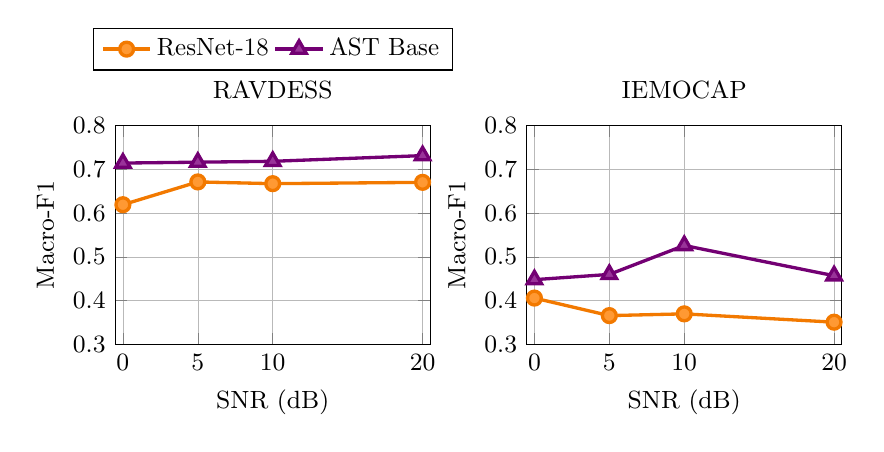
\begin{tikzpicture}
    \pgfplotsset{compat=1.18}

    \begin{groupplot}[
      group style={group size=2 by 1, horizontal sep=3.5em},
      width=0.46\textwidth, height=0.36\textwidth,
      xmin=-0.5, xmax=20.5,
      ymin=0.30, ymax=0.80,
      xtick={0,5,10,20},
      xlabel={SNR (dB)}, ylabel={Macro-F1},
      grid=both,
      grid style={line width=.1pt, draw=gray!30},
      major grid style={line width=.2pt, draw=gray!55},
      ticklabel style={font=\small},
      label style={font=\small},
      ytick distance=0.1
    ]

    % ---------- RAVDESS ----------
    \nextgroupplot[title={RAVDESS}, title style={font=\small},
      legend style={nodes={scale=0.9, transform shape}, at={(0.5,1.25)}, anchor=south, legend columns=2}
    ]
    \addplot+[very thick, color=orange!95!black, mark=*, mark size=2.5pt, mark options={fill=orange!80!white}]
      coordinates {(0,0.619) (5,0.671) (10,0.667) (20,0.670)};
    \addlegendentry{ResNet-18}

    \addplot+[very thick, color=violet!90!black, mark=triangle*, mark size=3pt, mark options={fill=violet!80!white}]
      coordinates {(0,0.714) (5,0.716) (10,0.718) (20,0.731)};
    \addlegendentry{AST Base}

    % ---------- IEMOCAP ----------
    \nextgroupplot[title={IEMOCAP}, title style={font=\small}]
    \addplot+[very thick, color=orange!95!black, mark=*, mark size=2.5pt, mark options={fill=orange!80!white}]
      coordinates {(0,0.406) (5,0.366) (10,0.370) (20,0.351)};
    \addplot+[very thick, color=violet!90!black, mark=triangle*, mark size=3pt, mark options={fill=violet!80!white}]
      coordinates {(0,0.448) (5,0.460) (10,0.526) (20,0.457)};

    \end{groupplot}
    \end{tikzpicture}
    \caption{Experiment D: Macro-F1 vs. SNR with natural soundscapes for ResNet-18 and AST Base.}
    \label{fig:snr_ablation_macroF1}
\end{figure}
% !TEX root =  ../Dissertation.tex

\chapter{Discussion}

\begin{enumerate}
    \item \textbf{Architecture–augmentation interaction} Across experiments, the transformer (AST Base) benefits from noise augmentation, whereas the CNN (ResNet-18) is more fragile to heterogeneous backgrounds. With ESC-50 noise, AST surpasses clean baselines on both datasets (RAVDESS Macro-F1: 0.734 vs. 0.714; IEMOCAP: 0.515 vs. 0.448), while ResNet-18 drops on RAVDESS (0.527 vs. 0.682). Under 20 dB white noise, AST preserves RAVDESS performance and raises Macro-F1 on IEMOCAP; ResNet-18 shows small degradations. These results suggest attention-based models absorb temporal–spectral perturbations better, whereas convolutional inductive biases can over-regularize fine structure under broad noise.

    \item \textbf{Precision–recall balance under dataset heterogeneity} IEMOCAP shows stronger class imbalance and session/speaker variability than RAVDESS, and augmentation shifts operating points differently. With ESC-50, AST trades a modest precision decrease (0.682$\to$0.645) for a recall gain (0.413$\to$0.488), raising Macro-F1 to 0.515 and improving coverage of minority or ambiguous emotions. ResNet-18 shows the opposite (precision 0.388$\to$0.519; recall 0.475$\to$0.327), lowering Macro-F1 to 0.323 and implying a conservative regime. On RAVDESS, both models keep precision–recall more balanced, indicating corpus complexity largely dictates calibration.

    \item \textbf{SNR sensitivity and non-monotonic trends} Under natural soundscapes (Experiment D), AST on RAVDESS improves slightly with SNR (Macro-F1 0.714$\to$0.731 from 0 to 20 dB), while on IEMOCAP it peaks at 10 dB (0.526) then declines at 20 dB (0.457), revealing a sweet spot where augmentation regularizes without oversuppressing cues. ResNet-18 varies little on RAVDESS (0.619–0.671) but degrades with increasing SNR on IEMOCAP (0.406 at 0 dB to 0.351 at 20 dB), consistent with increased conservativeness. Overall, robustness depends on SNR and dataset variability; mid-SNR mixes often best balance invariance and separability for AST.
\end{enumerate}
% !TEX root =  ../Dissertation.tex

\chapter{Conclusion}

This dissertation set out to investigate and improve the performance of Speech Emotion Recognition systems, with a specific focus on enhancing model robustness in noisy environments. Through a systematic series of experiments, we conducted a comparative analysis of multiple feature representations (MFCCs and Mel-spectrograms) and four distinct deep learning architectures: MLP, a shallow CNN, ResNet-18, and the Audio Spectrogram Transformer (AST). The central contribution of this work lies in the extensive evaluation of on-the-fly noise augmentation as a mechanism for improving generalization, using both the RAVDESS and IEMOCAP datasets as testbeds. The main findings and their implications are summarized below.

The experimental results provide conclusive evidence for the architectural superiority of the Audio Spectrogram Transformer. Across all conditions, AST consistently outperformed the other models, achieving the highest accuracy and macro-F1 scores on both clean and noise-augmented test sets. This highlights the effectiveness of its self-attention mechanism in capturing global spectro-temporal dependencies that are crucial for emotion discrimination. Furthermore, on-the-fly noise augmentation proved to be a powerful and effective regularizer. For the AST model, training with a diverse set of natural soundscapes not only fortified its performance against noise but also led to improved results on the original clean data, suggesting that the perturbations encouraged the model to learn more generalizable and salient affective features.


A key insight from this work is the strong interaction between model architecture and the augmentation strategy. The benefits of augmentation were most pronounced for the AST model, which successfully absorbed the acoustic variability to enhance its representations. In contrast, the ResNet-18 architecture, despite its depth, showed fragility and performance degradation when exposed to the same heterogeneous noise, indicating that its convolutional inductive biases may be less suited for disentangling emotional content from complex background sounds. This dissertation also confirmed that performance is highly dependent on dataset characteristics; on the more challenging and spontaneous IEMOCAP dataset, augmentation prompted the AST model to achieve a better precision-recall balance, improving its ability to recognize ambiguous or minority-class emotions.


While this study provides a clear direction for robust SER, several limitations present avenues for future research. The noise sources, though representative, were limited to white noise and a subset of the ESC-50 dataset; future work could incorporate a wider variety of real-world noises, such as babble, music, and channel reverberation. Additionally, while AST proved effective, its performance could be further enhanced by leveraging self-supervised pre-training on large-scale unlabeled datasets, following frameworks like wav2vec 2.0. Another promising direction is the extension of this framework to multimodal SER, integrating textual or visual information, which is particularly relevant for conversational datasets like MELD. Finally, future investigations could explore model interpretability to better understand how attention mechanisms identify and leverage emotionally salient regions within a spectrogram. In summary, the findings of this thesis provide compelling evidence for the adoption of transformer-based architectures combined with robust data augmentation for building the next generation of effective and reliable Speech Emotion Recognition systems.







\bibliographystyle{abbrv}
\bibliography{bibliography}


\include{Appendices/Appendices}

\end{document}
